\section{Service Mesh}
\subsection{Microservices}
A microservice is a small, independent application that handles one specific business function and communicates with other services via APIs. This approach breaks large applications into smaller, loosely-coupled services that can be developed and deployed independently. Opposite of a Monolith.
\subsection{Challenges}
\textbf{Communication:} Services need to know all the endpoints of services they have to communicate with. A new microservice can result in many changes in existing services.
\textbf{Security:} Communication in cluster is not secured, every service can talk to every other service in a cluster. Possible attackers have full access.
\textbf{Monitoring:} Since services are spread out, monitoring can be tedious. Non Business logic must be added to each application, adds complexity.
\subsection{Service Mesh w/ Sidecar Pattern}
A Service Mesh uses Sidecars in all the Pods. The sidecars act as a proxy and also include additional functionality (Monitoring, Security, ...)

% TODO: pros/cons

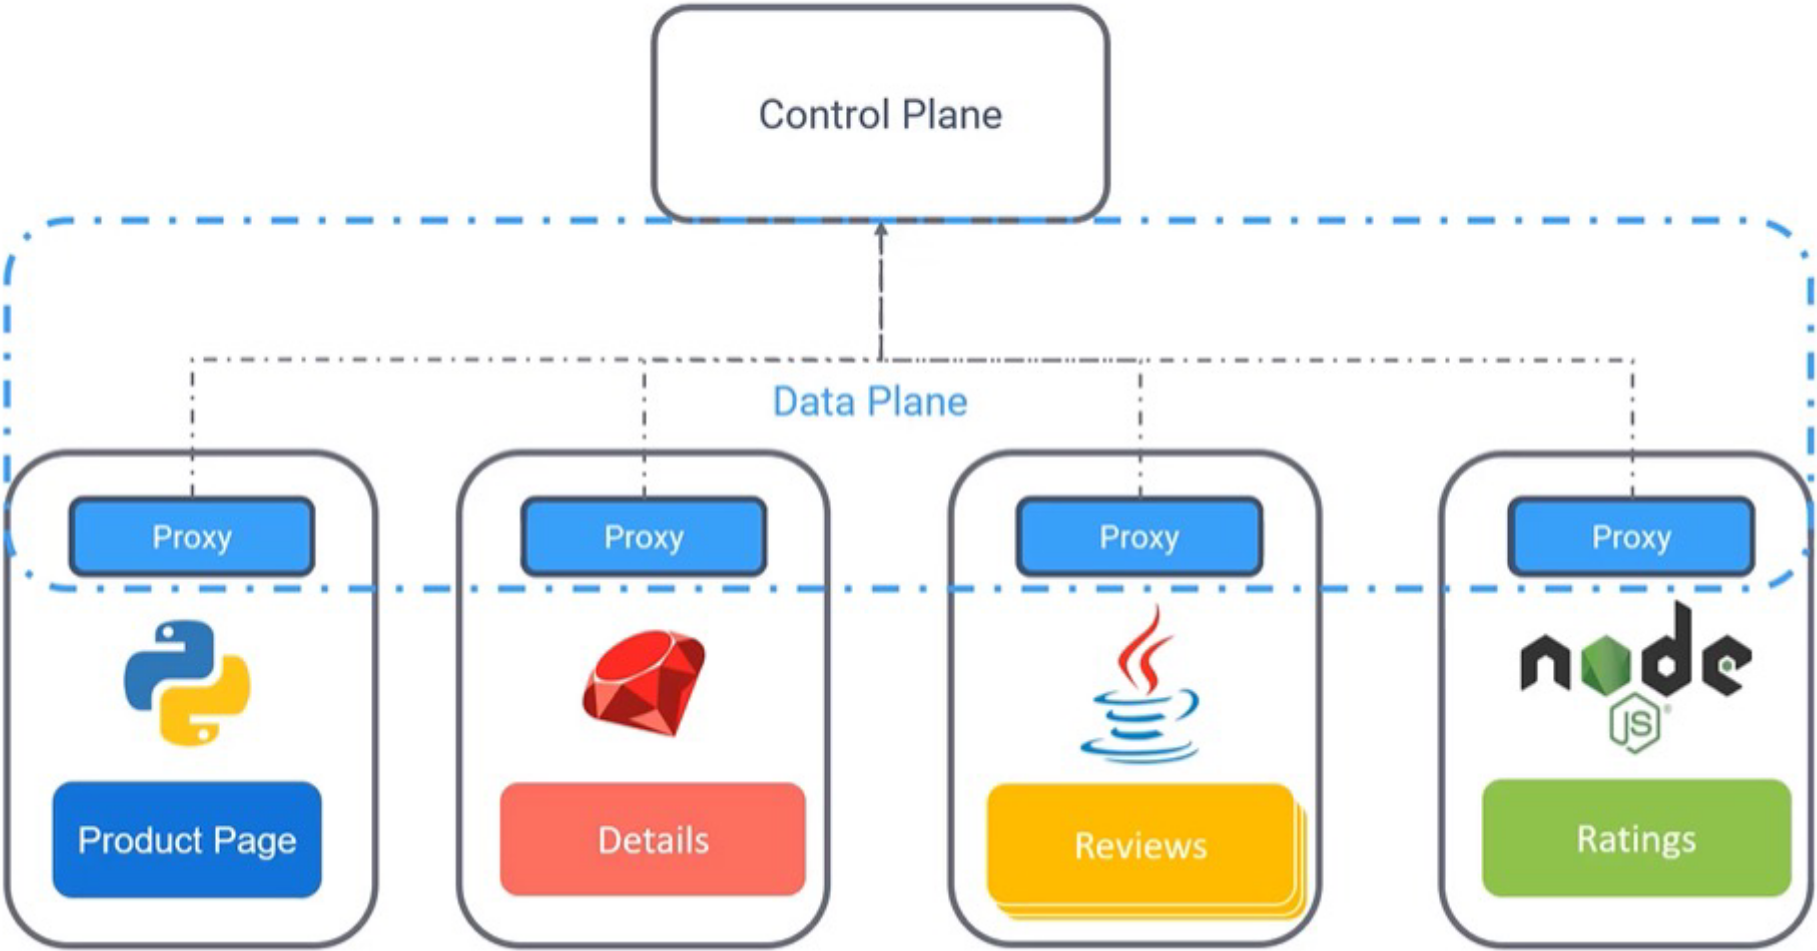
\includegraphics[width=0.19\textwidth]{ServiceMesh.png}

The two key components of a service mesh are:
\textit{Data Pane:} Consists of sidecar-proxies in pods which handle communication etc. (Example: Envoy)
\textit{Control Pane:} Manages and distributes configuration to data pane. (Example: Istiod)

Envoy proxies in each pod authenticate each other via \textbf{mTLS} (mutual TLS: client and server authenticate each other using TLS certificates)

\subsection{Ambient Mesh}
The Traffic Mesh with Sidecar pattern comes with some downsides: It is invasive, can lead to overallocation of resources per pod, breaks traffic.

Ambient mesh solves this by removing the sidecar proxies, rather providing one zTunnel per node. These zTunnels communicate with across nodes. They operate on Layer 4. zTunnels also authenticate each other using mTLS.

Additionally, optionally L7 waypoint proxies can be used for policy enforcements.

\subsection{Traffic Management}
In istio, K8 ingress/egress are replaced by gateways, as they allow for more control.
A VirtualService binds to a gateway and determines how traffic is routed to services.
DestinationRules allow to
\begin{lstlisting}[language=yaml]
apiVersion: networking.istio.io/v1beta1
kind: Gateway
metadata:
  name: my-gateway
spec:
  selector:
    istio: ingressgateway
  servers:
  - port:
      number: 80
      name: http
      protocol: HTTP
    hosts:
    - "example.com"
--
apiVersion: networking.istio.io/v1beta1
kind: VirtualService
metadata:
  name: my-vs
spec:
  hosts:
  - "example.ch" # must match a gateway host
  gateways:
  - my-gateway
  http:
  - route:
    - destination:
        host: my-service
        weight: 99 # if a second destination is defined, weight can be used to split traffic accordingly
        port:
          number: 80
--
apiVersion: networking.istio.io/v1beta1
kind: DestinationRule
metadata:
  name: my-dr
spec:
  host: my-service
  trafficPolicy:
    tls:
      mode: ISTIO_MUTUAL
\end{lstlisting}

\subsection{Service Resiliency}
Istio allows for:
\textbf{Fault Injection:} Simulate networking failures to test error-handling.
\textbf{Timeouts:} Times out requests after a certain time to avoid queuing up a lot of requests.
\textbf{Retries:} Configure services to retry if another service cannot be reached.

Istio also allows all the CD\&D Deployment Strategies (see \textit{General Definitions})

Istio provides and exports Prometheus metrics per default.

\subsection{Security}
\textbf{Authentication:} Services use mTLS to authenticate each other. \\
\textbf{Authorization:} Using AuthorizationPolicies, we get Fine-grained access control using Role-based access control (RBAC).

\begin{lstlisting}[language=yaml]
# Namespace-wide mTLS enforcement using PeerAuthentication
apiVersion: security.istio.io/v1beta1
kind: PeerAuthentication
metadata:
  name: default
  namespace: production  # Replace with your target namespace
spec:
  mtls:
    mode: STRICT
--
apiVersion: security.istio.io/v1beta1
kind: AuthorizationPolicy
metadata:
  name: require-jwt
  namespace: foo
spec:
  selector:
    matchLabels:
      app: httpbin # applies to these pods in namespace foo
  action: ALLOW
  rules:
  - from:
    - source:
        namespaces: ["frontend"] # allows traffic from frontend NS
    to:
    - operation:
        methods: ["GET"]
        paths: ["/headers"] # allows traffic to
\end{lstlisting}
